\section{Kết quả và thảo luận}\label{sec:results}

Toàn bộ số liệu trong phần này do chương trình của báo cáo chạy thực tế trên máy cá nhân (CPU), với cấu hình và seed cố định trong mã nguồn; khác với các phần trước, đây KHÔNG phải số liệu của tác giả hai paper.

\subsection{Thí nghiệm 1: chất lượng chọn ngữ cảnh}

\begin{table}[t]
\centering
\caption{Thí nghiệm 1 -- trung bình trên 200 mẫu HotpotQA, 5 tác tử, quét số vòng $T$ (giá trị ở $T{=}1$ và $T{=}6$). ``Tokens'' là số từ trong ngữ cảnh được chọn (lịch sử đầy đủ dài 524 từ ở $T{=}1$ và 5190 từ ở $T{=}6$). Answer-acc là tỷ lệ nhận đúng đáp án trong 8 ứng viên của bộ ghép từ vựng.}
\label{tab:exp1-rounds}
\begin{tabular}{l rr rr r}
\toprule
 & \multicolumn{2}{c}{$T=1$} & \multicolumn{2}{c}{$T=6$} & \\
\cmidrule(lr){2-3}\cmidrule(lr){4-5}
Chiến lược & Ev-F1 & Tokens & Ev-F1 & Tokens & Answer-acc \\
\midrule
full      & 0,289 & 524 & 0,297 & 5190 & 0,965--0,980 \\
window    & 0,289 & 524 & 0,172 & 1177 & 0,930--0,975 \\
semantic  & 0,264 & 29  & 0,260 & 295  & 0,870--0,880 \\
radar     & 0,232 & 23  & 0,157 & 146  & 0,870--0,890 \\
\bottomrule
\end{tabular}
\end{table}

\begin{figure}[t]
\centering
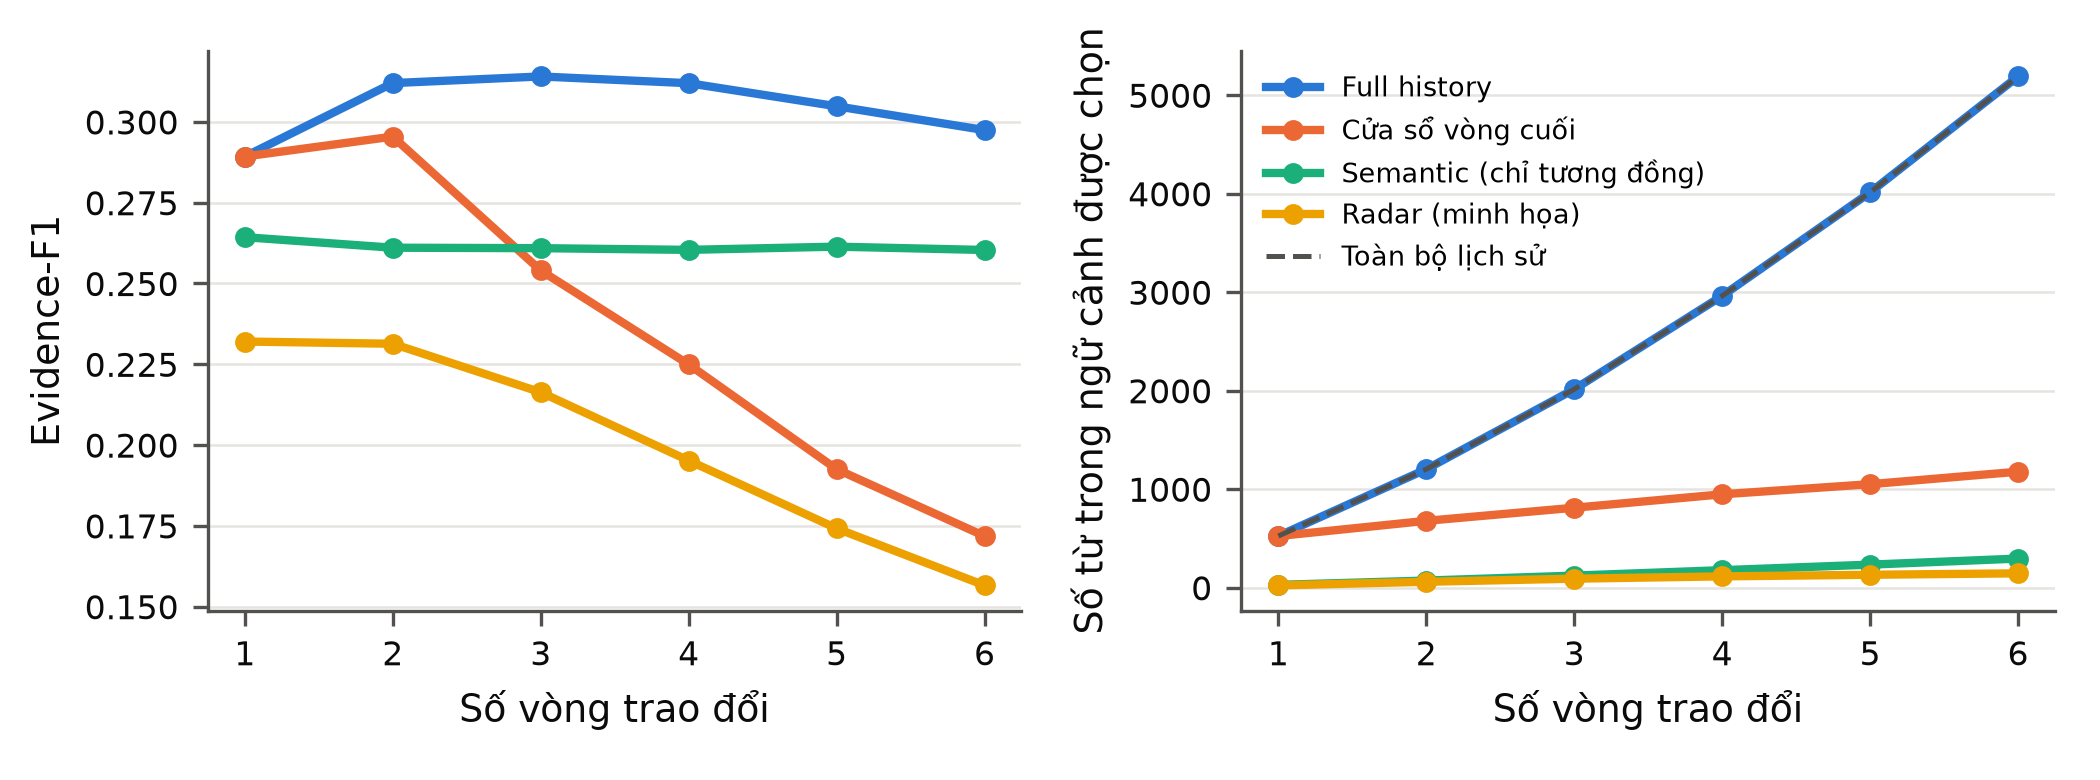
\includegraphics[width=\linewidth]{figures/exp1_rounds.png}
\caption{Thí nghiệm 1 theo số vòng trao đổi (200 mẫu HotpotQA, 5 tác tử). Trái: Evidence-F1 của ngữ cảnh được chọn so với supporting facts. Phải: số từ trong ngữ cảnh được chọn so với toàn bộ lịch sử (nét đứt). Số liệu do chương trình của báo cáo đo.}
\label{fig:exp1-rounds}
\end{figure}

Bảng~\ref{tab:exp1-rounds} và hình~\ref{fig:exp1-rounds} cho thấy ba điều. Thứ nhất, hiện tượng pha loãng xuất hiện đúng như paper mô tả: với chiến lược \texttt{full}, lịch sử phình từ 524 lên 5190 từ khi $T$ tăng từ 1 đến 6, precision của bằng chứng trong lịch sử giảm dần (từ 0,171 xuống 0,177 sau khi qua đỉnh), và Evidence-F1 đi ngang rồi giảm. Thứ hai, hai chiến lược lọc theo ngưỡng nén ngữ cảnh mạnh (radar giữ 146 từ trên 5190 từ lịch sử ở $T{=}6$, tỷ lệ $\approx$ 2,8\%) và tăng precision gấp khoảng đôi (0,33 so với 0,18), nhưng cái giá là recall: \texttt{radar} chỉ giữ lại 11\% bằng chứng vàng ở $T{=}6$. Thứ ba, chỉ số answer-acc của bộ ghép từ vựng đơn giản giảm rõ khi chuyển từ ngữ cảnh đầy đủ (0,965--0,980) sang ngữ cảnh lọc chặt (0,870--0,890).

Điểm thứ ba đáng dừng lại vì nó như là hình ảnh phản chiếu của một kết quả ablation trong paper gốc: Agent-Radar thử bỏ phần lái attention (chỉ nối các câu được chọn vào prompt) và thấy MuSiQue giảm từ 39,72 xuống 35,27 -- chọn ngữ cảnh thôi là chưa đủ. Thí nghiệm của báo cáo này không có bước lái attention (vì không chạy LLM), nên \texttt{radar} ở đây tương đương với đúng biến thể ablation đó: bộ chọn hoạt động đúng công thức, nhưng khi dùng như bộ lọc cứng thì mọi thông tin bị lọc bỏ là mất hẳn, và một bộ đọc yếu không bù lại được. Điều này củng cố thiết kế của paper gốc: giữ nguyên lịch sử và chỉ khuếch đại attention, thay vì xóa.

So trực tiếp \texttt{radar} với \texttt{semantic} (cùng ngưỡng $\theta=0{,}65$): hai hệ số suy giảm làm volume được chọn nhỏ đi (146 so với 295 từ ở $T{=}6$) nhưng không tăng precision, mà còn giảm recall (0,111 so với 0,221). Nguyên nhân nằm ở môi trường mô phỏng: nhiễu được phân bổ đều giữa các tác tử và thậm chí dày hơn ở các vòng sau (số câu nhiễu tăng theo $t$), nên vị trí không gian/thời gian ở đây hầu như không mang thông tin về chất lượng của câu -- suy giảm theo hop và theo tuổi chỉ ``trừ điểm'' thêm cho cosine. Trong hệ MAS thật mà paper xét, thông điệp xa và cũ ít đáng tin hơn, và đó là điều kiện để hai hệ số này phát huy tác dụng; môi trường mô phỏng đơn giản của báo cáo không tái tạo được điều kiện đó.

Thí nghiệm 1b kiểm chứng riêng vai trò \emph{xếp hạng} của hai hệ số suy giảm bằng cách cho mọi chiến lược chọn đúng $k$ câu (loại bỏ yếu tố ngưỡng). Kết quả: ở mọi mức $k \in \{10, 20, 40\}$, Evidence-F1 của xếp hạng có suy giảm thấp hơn chút ít so với xếp hạng thuần ngữ nghĩa (0,481 so với 0,495 tại $k{=}10$; 0,569 so với 0,584 tại $k{=}20$) -- cũng là hệ quả của việc vị trí không mang thông tin trong mô phỏng. Ngược lại, answer-acc ở $k{=}40$ nghiêng về \texttt{radar} (0,810 so với 0,785): tập được chọn ít trùng lặp hơn nên bộ ghép từ vựng nhận diện đáp án tốt hơn. Hai chiều đo cho hai kết quả khác dấu -- đây là chi tiết trung thực cần báo cáo thay vì chọn lọc cái thuận lợi.

\begin{figure}[t]
\centering
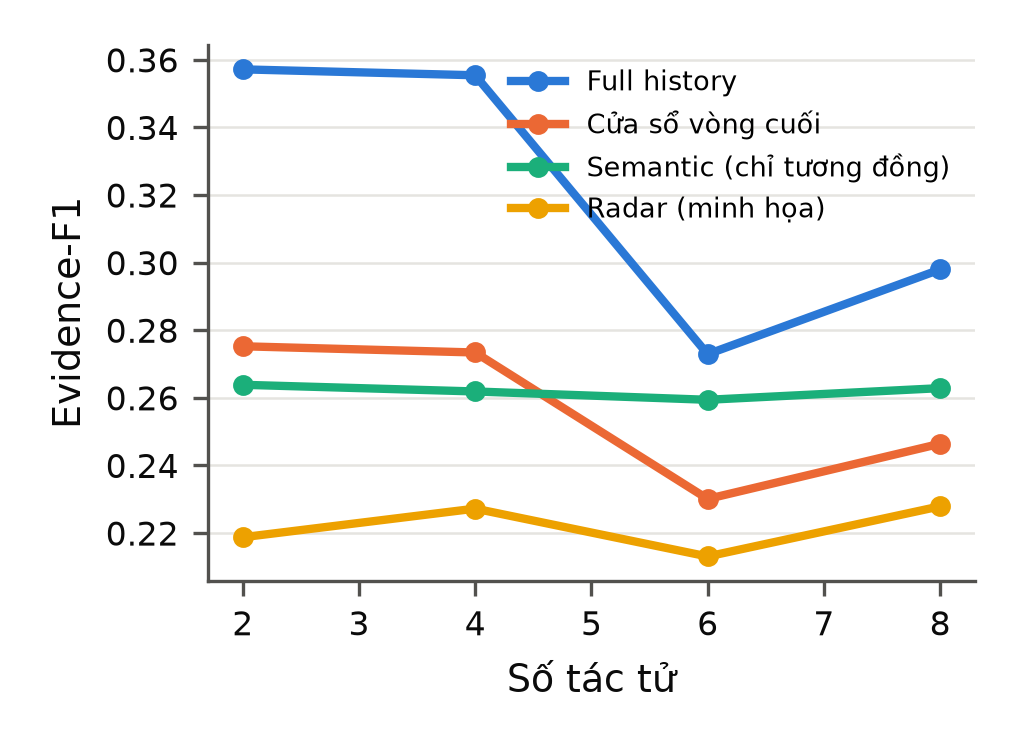
\includegraphics[width=\linewidth]{figures/exp1_agents.png}
\caption{Thí nghiệm 1 theo số tác tử ($T{=}3$). Evidence-F1 của \texttt{full} giảm khi thêm tác tử (pha loãng), còn các chiến lược lọc theo ngưỡng ổn định. Số liệu do chương trình của báo cáo đo.}
\label{fig:exp1-agents}
\end{figure}

Theo số tác tử (hình~\ref{fig:exp1-agents}), Evidence-F1 của \texttt{full} giảm từ 0,357 (2 tác tử) xuống 0,273 (6 tác tử) rồi hơi phục hồi (0,298 ở 8 tác tử) -- xu hướng ``thêm tác tử thì loãng hơn'' phù hợp với hiện tượng paper gốc mô tả ở Figure 2. Các chiến lược lọc theo ngưỡng gần như phẳng vì chúng chấm điểm theo truy vấn chứ không theo số nguồn. Thời gian chọn ngữ cảnh rất nhỏ ở mọi chiến lược (dưới 0,1 giây mỗi mẫu trên CPU; phần lớn thời gian thuộc về mã hóa câu), nên chi phí của bộ chọn không phải rào cản ở quy mô này.

\subsection{Thí nghiệm 2: DAIN đơn giản hóa trên ENRICO}

\begin{table}[t]
\centering
\caption{Thí nghiệm 2 -- accuracy trên tập test ENRICO (292 mẫu, 20 lớp; trung bình $\pm$ độ lệch chuẩn qua 5 seed, cấu hình huấn luyện giống §4.1 paper DAIN). $\bar{\tau}$: số tác tử kích hoạt trung bình; $\bar{\rho}$: mật độ đồ thị giao tiếp. Số liệu do chương trình của báo cáo đo.}
\label{tab:exp2-main}
\begin{tabular}{l rr r}
\toprule
Mô hình & Accuracy (\%) & $\bar{\tau}$/8 & $\bar{\rho}$ \\
\midrule
Early Fusion & \textbf{42,81} $\pm$ 0,57 & -- & -- \\
Late Fusion  & 41,58 $\pm$ 1,07 & -- & -- \\
Static MoE   & 39,79 $\pm$ 1,52 & 8,0 & -- \\
Sparse MoE   & 38,56 $\pm$ 1,69 & 4,0 & -- \\
DAIN-Static  & 35,14 $\pm$ 1,94 & 8,0 & 0,434 \\
DAIN-NoComm  & 37,81 $\pm$ 0,93 & 4,0 & 0,308 \\
DAIN (full)  & 38,56 $\pm$ 1,26 & 4,0 & 0,389 \\
\bottomrule
\end{tabular}
\end{table}

\begin{figure}[t]
\centering
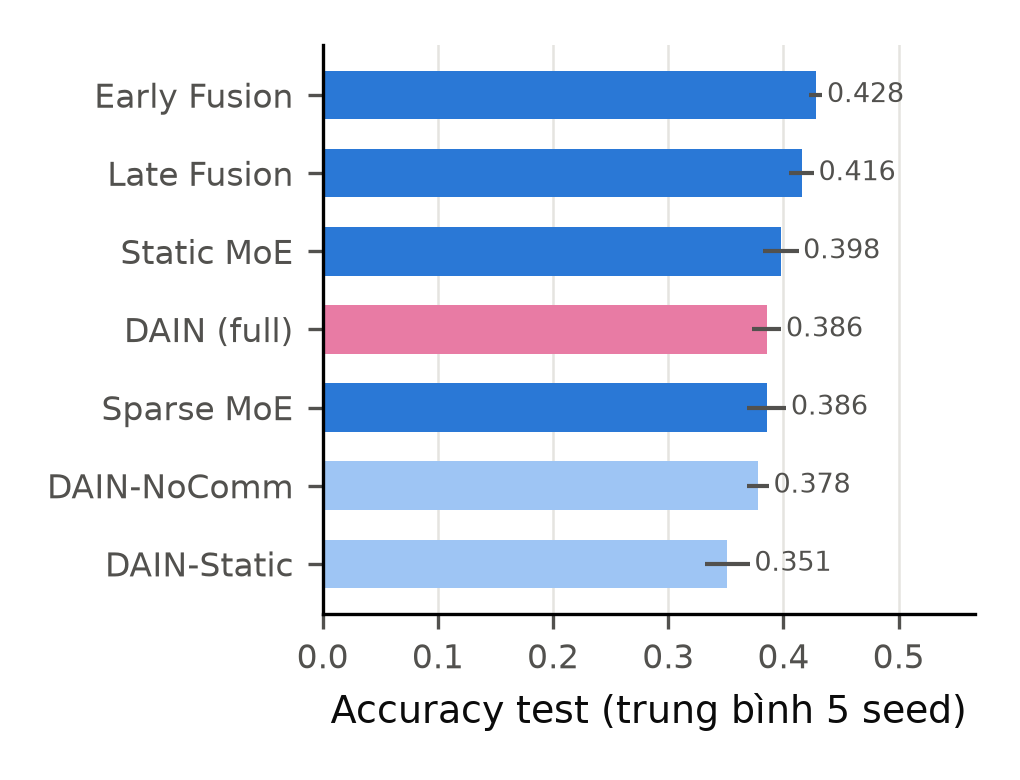
\includegraphics[width=\linewidth]{figures/exp2_main.png}
\caption{Thí nghiệm 2: accuracy trung bình qua 5 seed (thanh lỗi: độ lệch chuẩn). Ba biến thể DAIN dùng màu khác nhóm baseline để dễ theo dõi thứ tự ablation. Số liệu do chương trình của báo cáo đo.}
\label{fig:exp2-main}
\end{figure}

Bảng~\ref{tab:exp2-main} và hình~\ref{fig:exp2-main} cho kết quả chia làm hai lớp. Trong nội bộ họ DAIN, thứ tự ablation khớp định tính với Table~4 của paper: mô hình đầy đủ (38,56\%) cao hơn biến thể bỏ giao tiếp (37,81\%), và cao rõ rệt hơn biến thể mọi tác tử luôn bật (35,14\%). Cơ chế điều phối cũng hoạt động đúng thiết kế: gate giữ đúng 4/8 tác tử kích hoạt, mật độ đồ thị giao tiếp $\bar{\rho} = 0{,}39$ thấp hơn đáng kể mức dày đặc (1,0), tức Meta-Controller tự tạo ra được cấu trúc thưa như paper mô tả.

Ngược lại, lợi thế của DAIN so với các baseline fusion tĩnh -- kết quả trung tâm của paper gốc -- \emph{không} xuất hiện trong thiết lập này: Early Fusion đơn giản dẫn đầu với 42,81\%. Mức chênh vượt quá một độ lệch chuẩn của các mô hình DAIN. Một thử nghiệm chẩn đoán với learning rate cao hơn (3e-4 và 1e-3) không thay đổi thứ tự này. Có ba nguyên nhân khả dĩ, đều nằm ở những gì báo cáo phải đơn giản hóa: (i) dữ liệu nhỏ (1022 mẫu train) khiến các thành phần phụ thêm của DAIN -- 8 nhánh agent, đồ thị giao tiếp, loss chuyên môn hóa -- trở thành nguồn quá khớp hơn là lợi thế; (ii) encoder nhẹ (CNN nhỏ + bag-of-words) làm các modality ít giàu thông tin hơn nhiều so với ResNet-50/BERT-base mà paper dùng, trong khi cơ chế synergy/uniqueness/redundancy của DAIN được thiết kế để khai thác tương tác giàu giữa các modality; (iii) kết quả của paper là trung bình trên năm bộ dữ liệu với encoder chuẩn hóa, trong khi báo cáo này chỉ chạy một bộ. Nói cách khác, thí nghiệm này xác nhận kiến trúc huấn luyện được và các cơ chế điều phối vận hành đúng, nhưng không xác nhận được tuyên bố hiệu năng của paper -- và báo cáo ghi nhận điều đó nguyên văn như vậy.

\begin{figure}[t]
\centering
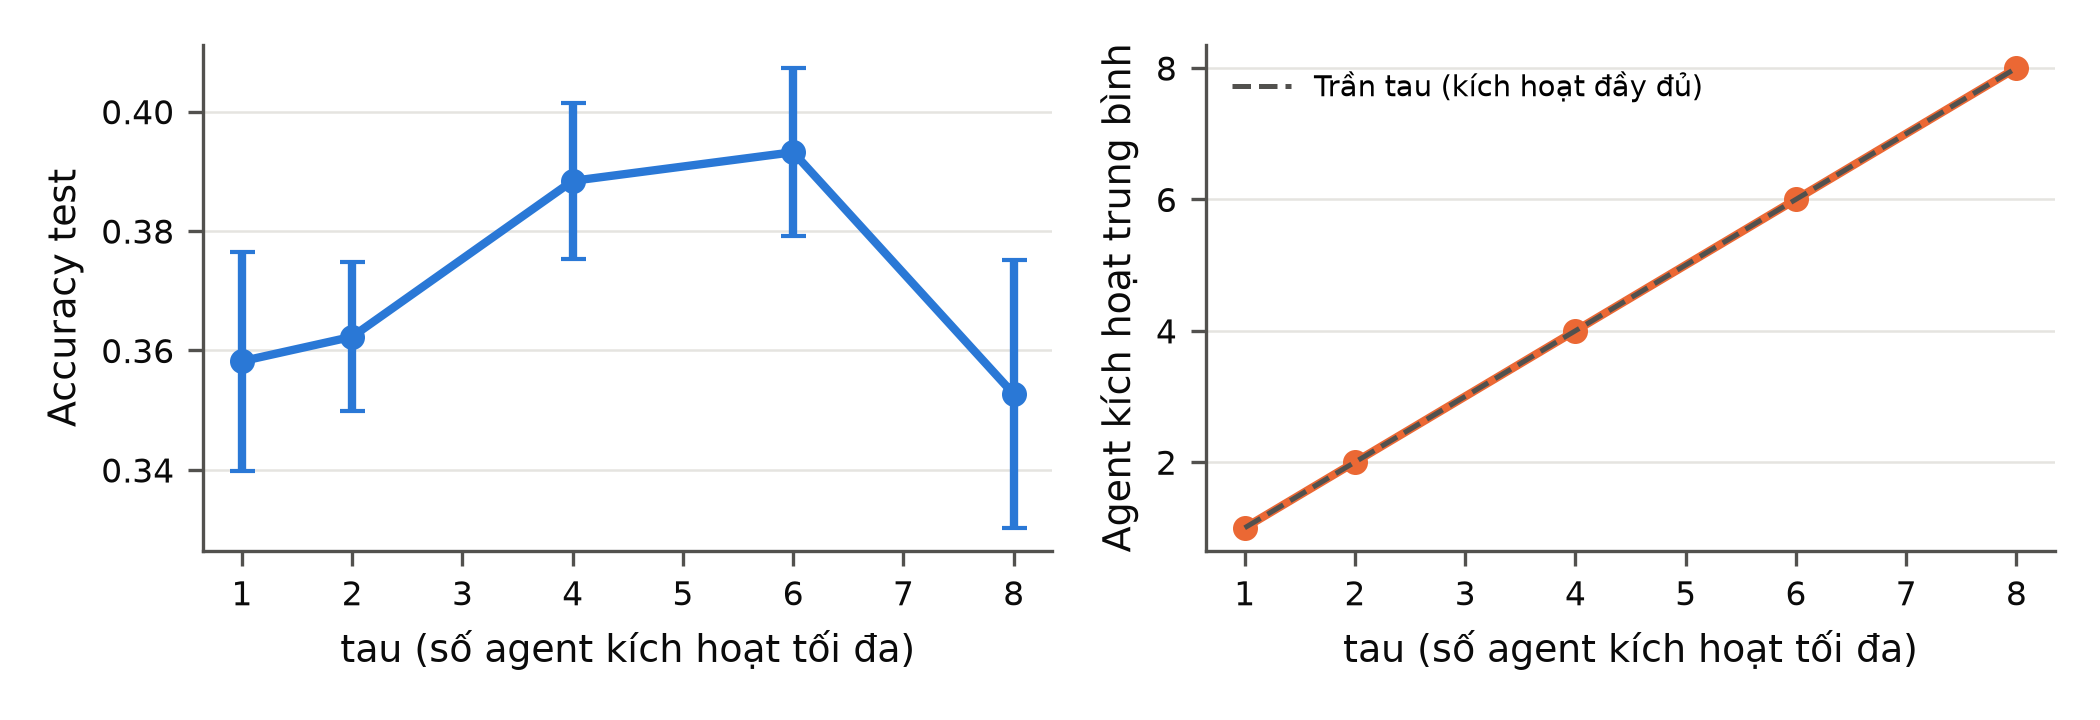
\includegraphics[width=\linewidth]{figures/exp2_tau.png}
\caption{Thí nghiệm 2: quét $\tau$ cho DAIN (trái: accuracy; phải: số tác tử kích hoạt trung bình so với trần $\tau$). Hiệu quả không đơn điệu theo $\tau$. Số liệu do chương trình của báo cáo đo.}
\label{fig:exp2-tau}
\end{figure}

Quét $\tau$ (hình~\ref{fig:exp2-tau}) cho kết quả không đơn điệu: accuracy tăng từ 35,82\% ($\tau{=}1$) lên đỉnh 39,32\% ($\tau{=}6$) rồi tụt xuống 35,27\% khi bật đủ 8 tác tử. Xu hướng ``quá ít tác tử thì thiếu, quá nhiều thì nhiễu'' khớp định tính với Table~5 của paper (đỉnh ở $\tau{=}4$, giảm nhẹ ở $\tau{=}8$), dù vị trí đỉnh khác đi -- một khác biệt nữa có thể quy về quy mô dữ liệu và encoder.

\subsection{Đối chiếu với paper gốc và giới hạn}
Tổng hợp lại: những gì hai thí nghiệm xác nhận được là (1) công thức chọn ngữ cảnh của Agent-Radar hoạt động đúng như mô tả và nén ngữ cảnh với mật độ bằng chứng cao gấp đôi baseline; (2) kết luận của paper rằng ``chọn ngữ cảnh phải đi kèm cơ chế đưa vào lúc suy luận'' thể hiện ngay cả trong một mô phỏng không có LLM; (3) thứ tự ablation của DAIN (full $>$ NoComm $>$ Static) và tính chất không đơn điệu theo $\tau$ tái hiện được ở quy mô nhỏ. Những gì không xác nhận được: lợi thế của DAIN so với baseline tĩnh trong thiết lập đơn giản hóa, và lợi thế của hai hệ số suy giảm trong môi trường mô phỏng nơi vị trí không mang thông tin. Các giới hạn khác đã nêu ở phần~\ref{sec:experiments}: thí nghiệm 1 là mô phỏng quy tắc chứ không phải hành vi LLM; thí nghiệm 2 thay encoder lớn và chỉ dùng 1/5 số bộ dữ liệu; và cả hai paper đều chưa có mã nguồn chính thức để đối chiếu.
